\section{Digital Representation of Continuous-time Systems and Filter Design} 

\subsection{The System}

To design the desired analogue filter as digital equivalent, aliasing is always the first thing to think of. In the case given in this assignment, the signal is already band limited and the sampling frequency is higher than the double of the band limit of the input signal. So it can be passed on applying further methods to prevent aliasing.


In this drawing shown in figure \ref{fig:draw}, the DAC is supposed to have already an analogue reconstruction filter implemented at the output.\\
In practical experience also the necessary processing times of the ADC and DAC must be taken into account, but as there are no further information on these devices, their processing times are supposed to be equal to zero.\\
As already mentioned that the input signal is band-limited, the discrete-time filter $H(e^{j\omega})$ is given by:

\begin{figure}[h]
\centering
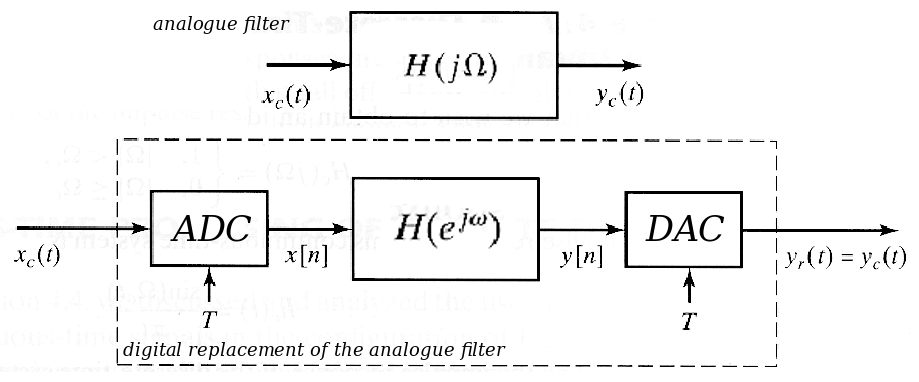
\includegraphics[width=\textwidth]{pics/drawing.png}
\caption{The discrete time system as equivalent to the analogue filter}
\label{fig:draw}
\end{figure}

\begin{equation}
H(e^{j \omega}) = H(j \Omega) |_{\Omega = \frac{\omega}{T}} = e^{-j\Omega \Delta T} |_{\Omega = \frac{\omega}{T}} = e^{-j \frac{\omega}{T} \Delta T} = e^{-j \omega \Delta}
\end{equation}

So the desired digital filter is an allpass filter with linear phase.


\subsection{The Filter Design}
\label{chap:filter_design}
For applying the filter design in a discrete environment like Matlab, the desired filter was sampled dense in the relevant band of the (normalized) frequency domain (from $-0.8\pi$ to $0.8\pi$, as it is defined by the error function). Frequencies outside this relevant band are also called "don't care band" and are not considered in the design process.\\
The Matlab script which was written to solve this task, tries filter orders $N$ in ascending order to determine the minimum filter order needed to fulfil the given constraint $||E(e^{j\omega})||_2 < -50dB$.\\
Because the desired filter which has to be approximated has an allpass characteristic, only even filter orders are considered as only these types of FIR filters are applicable for both low and high pass designs.\\
As additional integer delay $N/2$ is considered because the chosen filter types impulse response has at $N/2$ its maximum (the output "impulse" is shifted by $N/2$ samples) and therefore with an integer delay of $N/2$ the maximum number of coefficients can be used to produce the output signal, which ensures the best approximation accuracy.\\
For the least squares design, a so called DTFT Matrix $F$ was generated for each filter order (also as a dense sampled version) which is used to calculate the coefficients of the FIR filter by a leftside multiplication of the sampled version of the desired frequency response with the pseudo inverse of that matrix. This operation determines automatically the least squares solution of the under-determined equation system laying behind.\\
At each trial with a different number of coefficients the error is evaluated and the script terminates when the constraint is fulfilled. To evaluate the error $||E(e^{j\omega})||_2$ the integral is approximated by the weighted sum of all discrete samples in the frequency domain. As weight, the frequency step between each sample is used.\\
By running the script, a minimum filter order of $N=6$ leading to an approximation error of $-54.62dB$ was determined.

\begin{figure}[h]
\centering
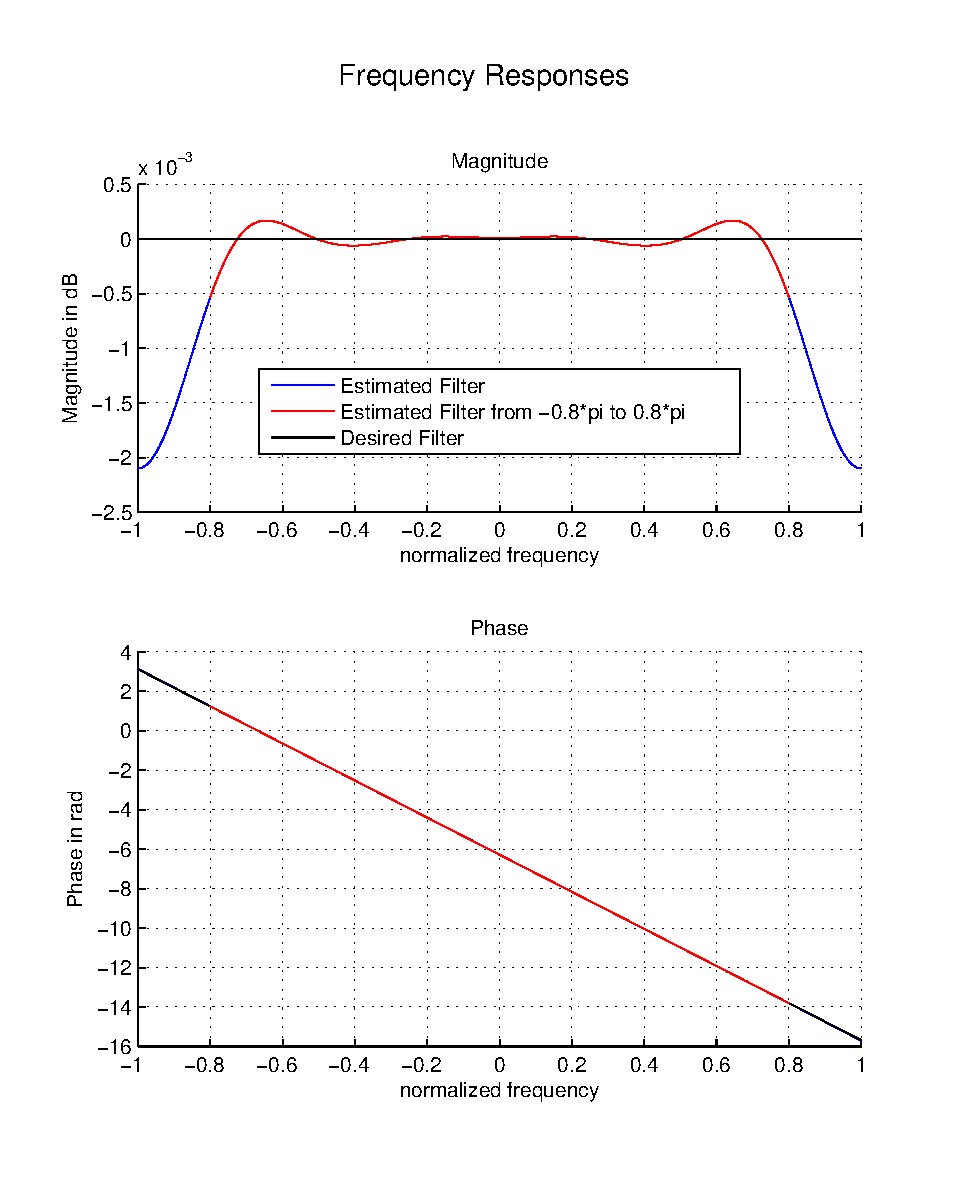
\includegraphics[width=\textwidth]{pics/fig1.eps}
\caption{The frequency responses of the design and the desired filter}
\label{fig:freqz}
\end{figure}

Figure \ref{fig:freqz} shows the frequency responses of the desired filter, the approximated filter with $N=6$ in the relevant band and the don't care band. As you can see, the linear phase can be matched perfectly, whereas the magnitudes are slightly different from the desired filter, especially around $-0.8\pi$ and $0.8\pi$. Additionally, the squared error in $dB$ over the normalized frequency is plotted in figure \ref{fig:error}. The maximum error (worst case) is located exactly at $-0.8\pi$ and $0.8\pi$ with a value of $-48.95dB$.

\begin{figure}[h]
\centering
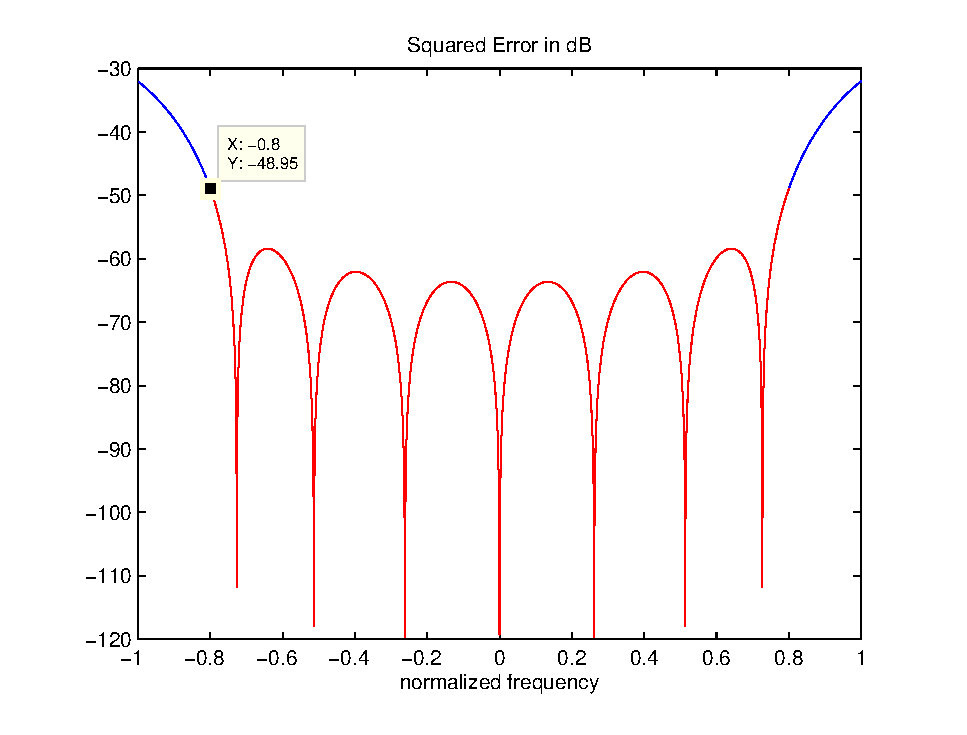
\includegraphics[width=\textwidth]{pics/fig2.eps}
\caption{The squared error of the filter design}
\label{fig:error}
\end{figure}

\subsection{Approximating the Coefficients by a Polynome}
\label{chap:poly}
Using the same procedure as in \ref{chap:filter_design}, for a given order of $N=10$ all FIR filter coefficients were determined and the fourth coefficient ($g_\Delta [3]$) was plotted, as shown in figure \ref{fig:coef3}.

The developed Matlab script is enables the user to try different polynomial orders for fitting the coefficients. In figure \ref{fig:coef3} also the determined polynome for a order $P=1$ is illustrated as black line, which already fits quite perfect. Using this script, also different orders can be calculated and visualised by simply changing one variable.\\
The coefficients for the determined polynome are $c_1 = 0.4044$ and $c_2 = 0.0000$.

\begin{figure}[h]
\centering
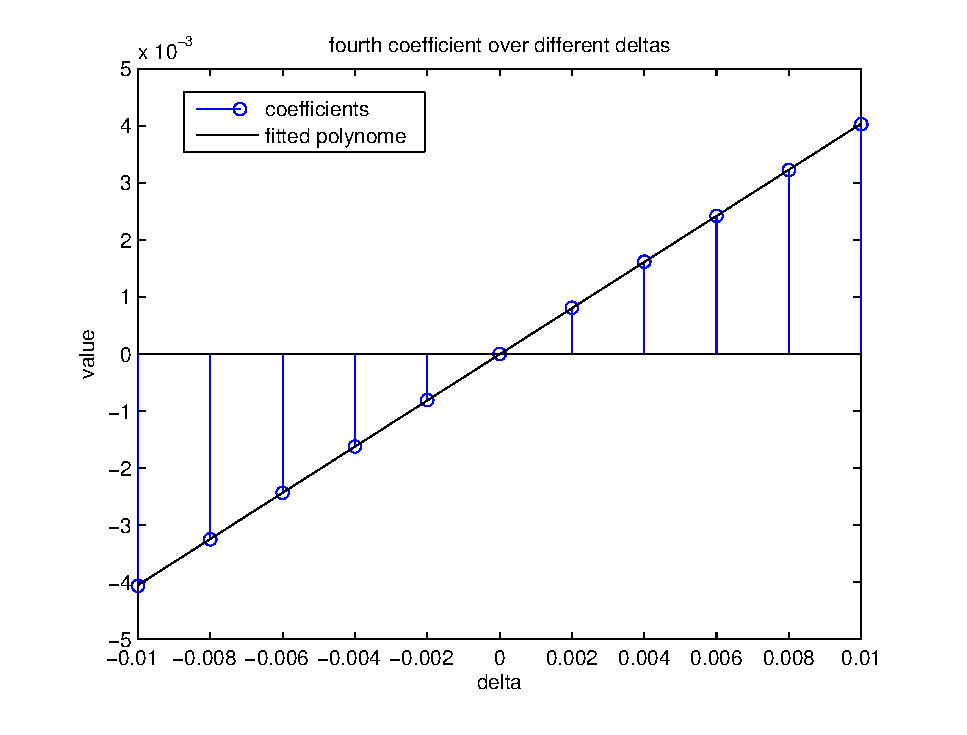
\includegraphics[width=\textwidth]{pics/fig4.eps}
\caption{The fourth coefficient and the approximated polynome}
\label{fig:coef3}
\end{figure}

\subsection{Farrow Filter}

For simplicity, the Matlab script in \ref{chap:poly} already calculates the coefficients of the polynomes for all the filter coefficients and stores them in the {\tt coeffs} matrix.\\
With this matrix we are able after generating the powers of the desired delta values to generate the desired impulse response by a simple matrix multiplication.\\
In order to compare the implicit design of the FIR filters to the design using Farrow filters, the absolute difference of each value of the two different impulse responses are taken into account.\\
Figure \ref{fig:impz} shows the absolute differences of the impulse responses over n for each value of $\Delta$ given in \ref{chap:poly}. All absolute errors are below $10^4$ which indicates that the Farrow design is absolute capable for this application.

\begin{figure}[h]
\centering
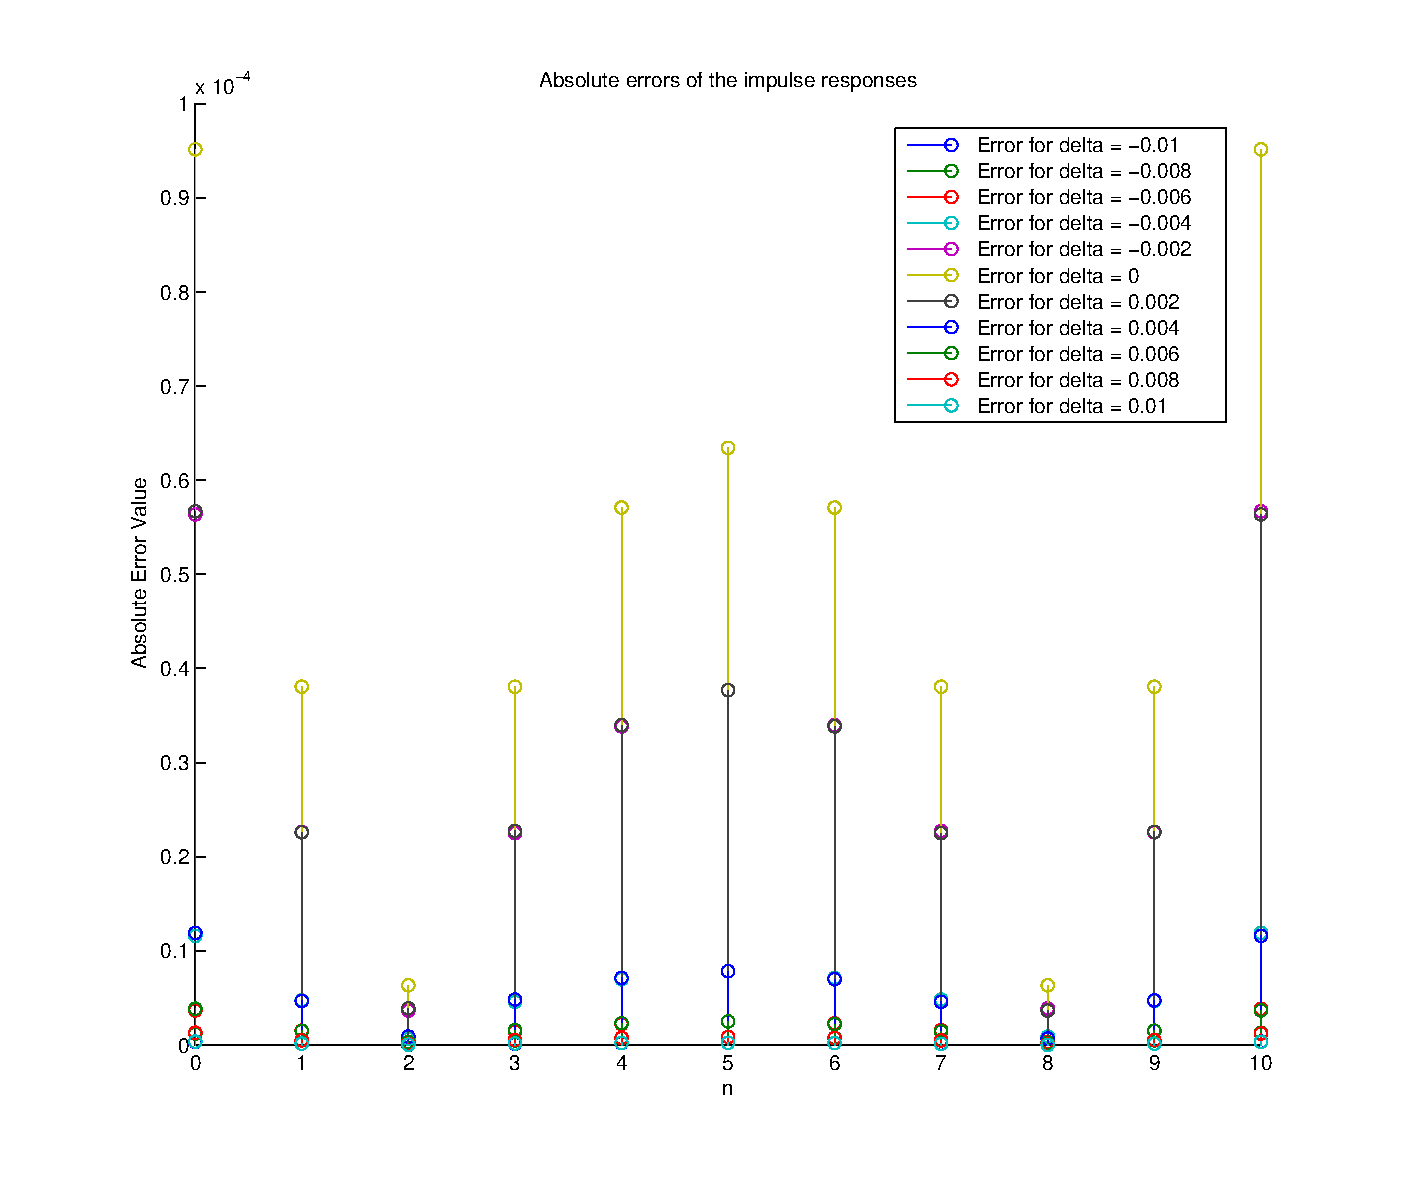
\includegraphics[width=\textwidth]{pics/fig5.eps}
\caption{Absolute Error of the impulse responses for the different deltas}
\label{fig:impz}
\end{figure}

